\section{15.10.2025}{Definicja powierzchni Riemanna}

Zaczynamy od pytania "jakie przestrzenie mogą być dziedzinami funkcji holomorficznej?"
W pierwszej kolejności poznajemy
\begin{enumerate}
  \item otwarty podzbiór płaszczyzny zespolonej, $U\subseteq\C$,
  \item otwarty podzbiór sfery Riemanna, $U\subseteq\RS$.
\end{enumerate}
Nie jest to jednak satysfakcjonująca nas odpowiedź.

\subsection{Dziedzina funkcji $\sqrt{z}$}

Rozważamy teraz konkretną funkcję, 
$$f(z)=\sqrt{z}=\sqrt{R}e^{i\theta/2}.$$ 

Wydaje się, że na $\C$ potrafimy znaleźć pierwiastek dla dowolnej liczby $z$. Jest to złudna uciecha, gdyż prowadzi nas do problemu z jednoznacznością. Wydaje się, że jeśli zaczniemy od $z=1$ i będziemy szli po okręgu jednostkowym zgodnie ze wskazówkami zegara i przeciwnie do wskazówek zegara to po połowie obrotu powinniśmy dojść do tej samej wartości pierwiastka. Tak jednak nie jest:
\begin{center}
  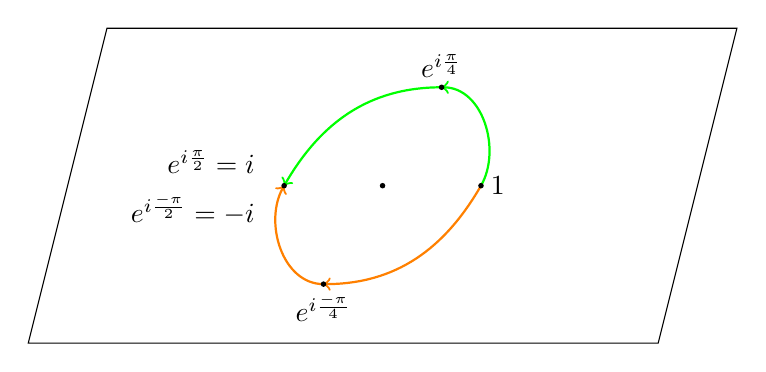
\begin{tikzpicture}
    \draw (-4, -2) -- (4, -2) -- (5, 2) -- (-3, 2) -- cycle;
    
    \draw[-> ,green, thick] (1.75, 0) to[out=60, in=0] (1.25, 1.25);
    \draw[-> ,green, thick] (1.25, 1.25) to[out=180, in=60] (-.75, 0);

    \draw[->, orange, thick] (1.75, 0) to[out=-120, in=0] 
                            (-.25, -1.25);
    \draw[->, orange, thick] (-.25, -1.25) to [out=180, in=-120]
                            (-.75, 0);

    \fill (0.5, 0) circle (1pt);
    \fill (1.75, 0) circle (1pt) node [right] {$1$};
    \fill (1.25, 1.25) circle (1pt) node [above] {$e^{i\frac{\pi}{4}}$};
    \fill (-.25, -1.25) circle (1pt) node [below] {$e^{i\frac{-\pi}{4}}$};
    \fill (-.75, 0) circle (1pt);
    \node[anchor=east] at (-1, .3) {$e^{i\frac{\pi}{2}}=i$};
    \node[anchor=east] at (-1, -.3) {$e^{i\frac{-\pi}{2}}=-i$};
  \end{tikzpicture}
\end{center}

Rozwiązaniem tego problemu jest wzięcie dwóch kopii $\C^*$, rozcięcie ich wzdłuż prostej $\R_-$, zdefiniowanie $\sqrt{z}$ na dwa różne sposoby na każdej i sklejenie ich na krzyż tak, aby $i$ było sklejone z $i$, a $-i$ z $-i$ (kolory).
\begin{center}
  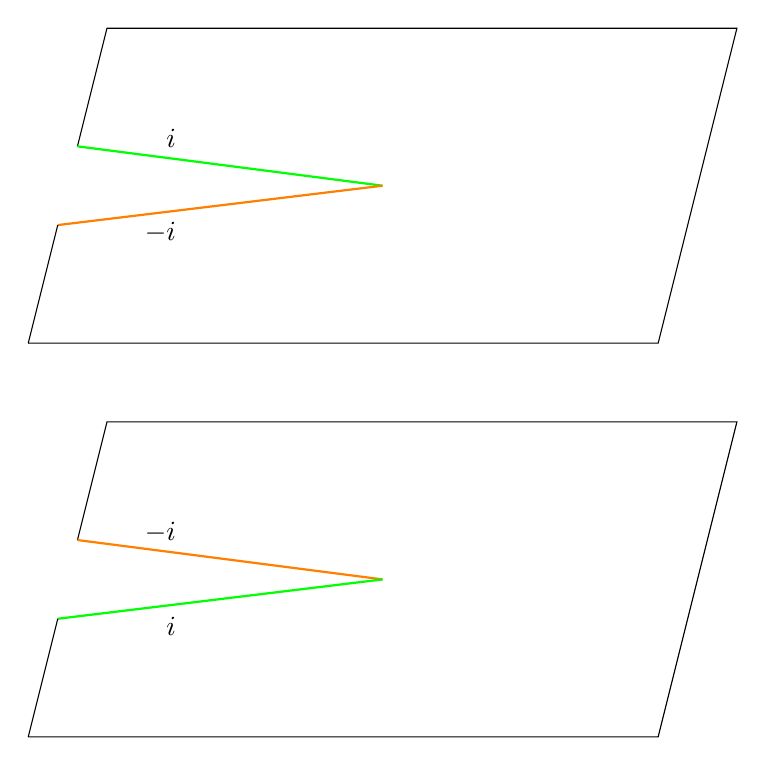
\begin{tikzpicture}
    \begin{scope}
      \draw (-4, -2) -- (4, -2) -- (5, 2) -- (-3, 2) -- (-3.375, .5);
      \draw[green, thick] (-3.375, .5) -- (0.5, 0);
      \draw[orange, thick] (.5, 0) -- (-3.625, -.5);
      \draw (-3.625, -.5) -- (-4, -2);
      \node[anchor=east] at (-2, .6) {$i$};
      \node[anchor=east] at (-2, -.6) {$-i$};
    \end{scope}

    \begin{scope}[shift={(0, -5)}]
      \draw (-4, -2) -- (4, -2) -- (5, 2) -- (-3, 2) -- (-3.375, .5);
      \draw[orange, thick] (-3.375, .5) -- (0.5, 0);
      \draw[green, thick] (.5, 0) -- (-3.625, -.5);
      \draw (-3.625, -.5) -- (-4, -2);
      \node[anchor=east] at (-2, .6) {$-i$};
      \node[anchor=east] at (-2, -.6) {$i$};
    \end{scope}
  \end{tikzpicture}
\end{center}

Na tej powierzchni $\sqrt{z}$ jest określony jednoznacznie.

\subsection{Definicja powierzchni Riemanna}







